\let\lesson\undefined
\newcommand{\lesson}{\phantomlesson{Bài 11: Ba định luật Newton về chuyển động}}
\chapter[Định luật III Newton]{Định luật III Newton}
\setcounter{section}{0}
\section{Lý thuyết}
\subsection{Định luật III Newton}
Khi vật $A$ tác dụng lên vật $B$ một lực, thì vật $B$ cũng tác dụng lại vật $A$ một lực. Hai lực này có điểm đặt lên hai vật khác nhau, có cùng giá, cùng độ lớn nhưng ngược chiều
$$\overrightarrow{F_{AB}}=-\overrightarrow{F_{BA}}$$
\begin{center}
	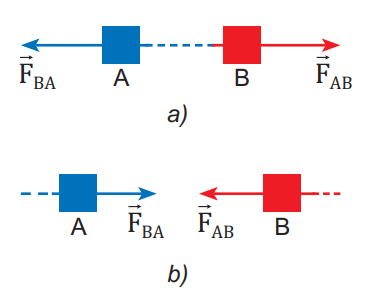
\includegraphics[width=0.3\linewidth]{../figs/VN10-2023-PH-TP017-1}
	\captionof{figure}{Cặp lực và phản lực}
\end{center}
Theo định luật III Newton, trong tương tác giữa hai vật, một lực gọi là lực tác dụng còn lực kia gọi là phản lực.
\subsection{Các đặc điểm của lực và phản lực}
\begin{itemize}
	\item Lực và phản lực luôn xuất hiện thành từng cặp (xuất hiện hoặc mất đi đồng thời).
	\item Lực và phản lực cùng tác dụng theo một đường thẳng (cùng giá), cùng độ lớn nhưng ngược chiều (hai lực như vậy gọi là hai lực trực đối).
	\item Lực và phản lực không cân bằng nhau (vì chúng đặt vào hai vật khác nhau).
	\item Cặp lực và phản lực là hai lực cùng loại.
\end{itemize}
\section{Mục tiêu bài học - Ví dụ minh hoạ}
\begin{dang}{Ghi nhớ định luật III Newton, \\đặc điểm của cặp lực - phản lực}
	\viduii{1}{Trong một vụ tai nạn, một ô tô tải đâm vào một ô tô con đang chạy ngược chiều. Ô tô nào chịu lực lớn hơn? Hãy giải thích.
	}
	{	\begin{center}
			\textbf{Hướng dẫn giải}
		\end{center}
		
		Theo định luật III Newton, ô tô tải tác dụng vào ô tô con một lực thì ô tô con cũng tác dụng ngược lại ô tô tải một lực. Hai ô tô chịu lực bằng nhau về độ lớn, cùng phương nhưng ngược chiều nhau. Vì vậy, hai ô tô đều chịu một lực có độ lớn bằng nhau.
		
	}
	\viduii{1}{Khi đi bộ xa hoặc leo núi, ta chống gậy thì đỡ mỏi  chân. Tại sao?
		
	}
	{	\begin{center}
			\textbf{Hướng dẫn giải}
		\end{center}
		
		Khi đi bộ hoặc leo núi, chân ta phải đạp vào mặt đất, đất sẽ tác dụng một phản lực làm cho ta đi về phía trước. Động tác đó lặp đi lặp lại nhiều lần khiến cho cơ chân bị mỏi. Nếu chống gậy, bên cạnh việc đạp vào mặt đất, ta còn dùng tay ấn mạnh gậy đẩy mặt đất về phía sau, mặt đất sẽ tác dụng vào đầu gậy một phản lực hướng về phía trước. Phản lực này sẽ truyền qua gậy đến cơ thể làm cho ta dịch chuyển về phía trước. Như vậy chân không còn chịu toàn bộ tác dụng của mặt đất lên cơ thể nên chân đỡ mỏi hơn.
	}
\end{dang}

\begin{dang}{Áp dụng định luật III Newton}
	\viduii{3}{Một quả bóng, khối lượng $\SI{500}{g}$ bay với tốc độ $\SI{20}{m/s}$ đập vuông góc vào bức tường và bay ngược lại với tốc độ $\SI{20}{m/s}$. Thời gian va đập  là $\SI{0,02}{s}$. Lực do bóng tác dụng vào tường có độ lớn và hướng như thế nào?		
	}
	{	\begin{center}
			\textbf{Hướng dẫn giải}
		\end{center}
		
		Chọn chiều dương chuyển động là chiều bóng bay đập vào tường.
		
		Gia tốc mà quả bóng đạt được là
		
		$$a = \dfrac{v-v_0}{t}=\dfrac{-\SI{20}{\meter/\second}-\SI{20}{\meter/\second}}{\SI{0.02}{\second}} = -\SI{2000}{\meter/\second^2}.$$
		
		Lực do tường tác dụng vào bóng là
		
		$$F =ma =\SI{0.5}{\kilogram}\cdot(\SI{-2000}{\meter/\second})= -\SI{1000}{\newton}.$$
		Dấu trừ cho thấy lực do tường tác dụng vào bóng ngược với chiều chuyển động ban đầu của bóng. 
		
		Theo định luật III Newton, lực do bóng tác dụng vào tường có cùng độ lớn là \SI{1000}{\newton}, nhưng có chiều ngược lại, tức là cùng chiều chuyển động ban đầu của bóng.	
	}
	\viduii{3}{Một A vật có khối lượng $\SI{1}{kg}$ chuyển động với tốc độ $\SI{5}{m/s}$ va chạm vào một vật B đứng yên. Sau va chạm vật A chuyển động ngược trở lại với tốc độ $\SI{1}{m/s}$, còn vật B chuyển động với tốc độ $\SI{2}{m/s}$. Hỏi khối lượng của vật B bằng bao nhiêu?
	}
	{	\begin{center}
			\textbf{Hướng dẫn giải}
		\end{center}
		
		Chọn chiều dương là chiều chuyển động ban đầu của vật A và gọi $\Delta t$ là thời gian va chạm giữa hai vật, đinh luật III Newton cho ta
		\begin{align*}
			\vec{F}_{AB}&=-\vec{F}_{BA}\\
			\Rightarrow\quad m_A\vec{a}_A&=-m_B\vec{a}_B\\
			\Rightarrow\quad m_A\dfrac{\Delta \vec{v}_A}{\Delta t}&=-m_B\dfrac{\Delta\vec{v}_B}{\Delta t}\\	
			\Rightarrow\quad m_A(v_A-v_{A0})&=-m_B(v_B-v_{B0})\\
			\Rightarrow\quad \SI{1}{\kilogram}\cdot(\SI{-1}{\meter/\second}-\SI{5}{\meter/\second})&=-m_B(\SI{2}{\meter/\second}-\SI{0}{\meter/\second})		
		\end{align*}
		Phương trình trên cho nghiệm $m_B = \SI{3}{kg}.$
		
	}
	
\end{dang}